\documentclass[9pt]{beamer}

% Beamer style
%\usetheme[secheader]{Madrid}
% \usetheme{CambridgeUS}
\useoutertheme{infolines}
\usecolortheme[rgb={0.65,0.15,0.25}]{structure}
% \usefonttheme[onlymath]{serif}
\beamertemplatenavigationsymbolsempty
%\AtBeginSubsection

% Packages
%\usepackage[french]{babel}
\usepackage[latin1]{inputenc}
\usepackage{color}
\usepackage{xspace}
%\usepackage{dsfont, stmaryrd}
\usepackage{amsmath, amsfonts, amssymb}
\usepackage{epsfig}
\usepackage{url}
\usepackage{/home/robin/LATEX/Biblio/astats}
%\usepackage[all]{xy}
\usepackage{graphicx}
\usepackage{tikz}

\input{/home/robin/RECHERCHE/EXPOSES/LATEX/Commands}

% Commands
\definecolor{darkred}{rgb}{0.65,0.15,0.25}
% \newcommand{\emphase}[1]{\textcolor{darkred}{#1}}
% \newcommand{\emphase}[1]{{#1}}
% \newcommand{\paragraph}[1]{\textcolor{darkred}{#1}}
% \newcommand{\refer}[1]{{\footnotesize{\textcolor{gray}{[{\cite{#1}}]}}}}
\newcommand{\Refer}[1]{{\footnotesize{\textcolor{gray}{[{#1}]}}}}
\renewcommand{\newblock}{}

% Symbols
\newcommand{\Abf}{{\bf A}}
\newcommand{\BM}{\text{BM}}
\newcommand{\betabf}{\text{\mathversion{bold}{$\beta$}}}
\newcommand{\Cbf}{{\bf C}}
\newcommand{\dd}{\xspace\text{d}}
% \newcommand{\Esp}{\mathbb{E}}
% \newcommand{\Ibb}{\mathbb{I}}
% \newcommand{\Cov}{\mathbb{C}\text{ov}}
\newcommand{\OU}{\text{OU}}
% \newcommand{\Var}{\mathbb{V}}
% \newcommand{\Hcal}{\mathcal{H}}
\newcommand{\Mcal}{\mathcal{M}}
% \newcommand{\Ncal}{\mathcal{N}}
\newcommand{\pa}{\text{pa}}
% \newcommand{\ra}{\emphase{\mathversion{bold}{$\rightarrow$}~}}
\newcommand{\Rbf}{{\bf R}}
\newcommand{\Scal}{\mathcal{S}}
\newcommand{\Xbf}{{\bf X}}
\newcommand{\Ybf}{{\bf Y}}
\newcommand{\Wbf}{{\bf W}}

% Directory
\newcommand{\fig}{../FIGURES}
%\newcommand{\figmotif}{/home/robin/RECHERCHE/RESEAUX/Motifs/FIGURES}


%====================================================================
%====================================================================

%====================================================================
%====================================================================
\begin{document}
%====================================================================
%====================================================================

%====================================================================
\title[Detection of adaptive shifts]{Inference of adaptive shifts for multivariate correlated traits}

\author[S. Robin]{P. Bastide, C. An�, \underline{S. Robin}, M. Mariadassou}

\institute[INRA/AgroParisTech/Paris-Saclay]{% INRA / AgroParisTech \\ ~\\
%  \vspace{-.1\textwidth}
  \begin{tabular}{ccccc}
    
\includegraphics[height=.06\textheight]{\fig/LogoINRA-Couleur} & 
    \hspace{.02\textheight} &
    
\includegraphics[height=.06\textheight]{\fig/logagroptechsolo} & 
    \hspace{.02\textheight} &
    
\includegraphics[height=.0633\textheight]{\fig/LogoParisSaclay}
    \\ 
  \end{tabular} \\
  \bigskip
  }

\date[Lake District, 2018]{StatScale meeting, Lake District, April 2018}

%====================================================================
%====================================================================
\maketitle
%====================================================================

%====================================================================
%====================================================================
\section{Modeling adaptive shifts}
\frame{\frametitle{Outline} \tableofcontents[currentsection]}
%====================================================================
\frame{\frametitle{Diversity of a trait}

  The diversity of a (multivariate) trait among a set of species results from:
  \begin{itemize}
   \item their shared history,
   \item potential %isolated shifts corresponding to 
   adaptive shifts due, e.g. to changes of ecological niche.
  \end{itemize}
  $$
  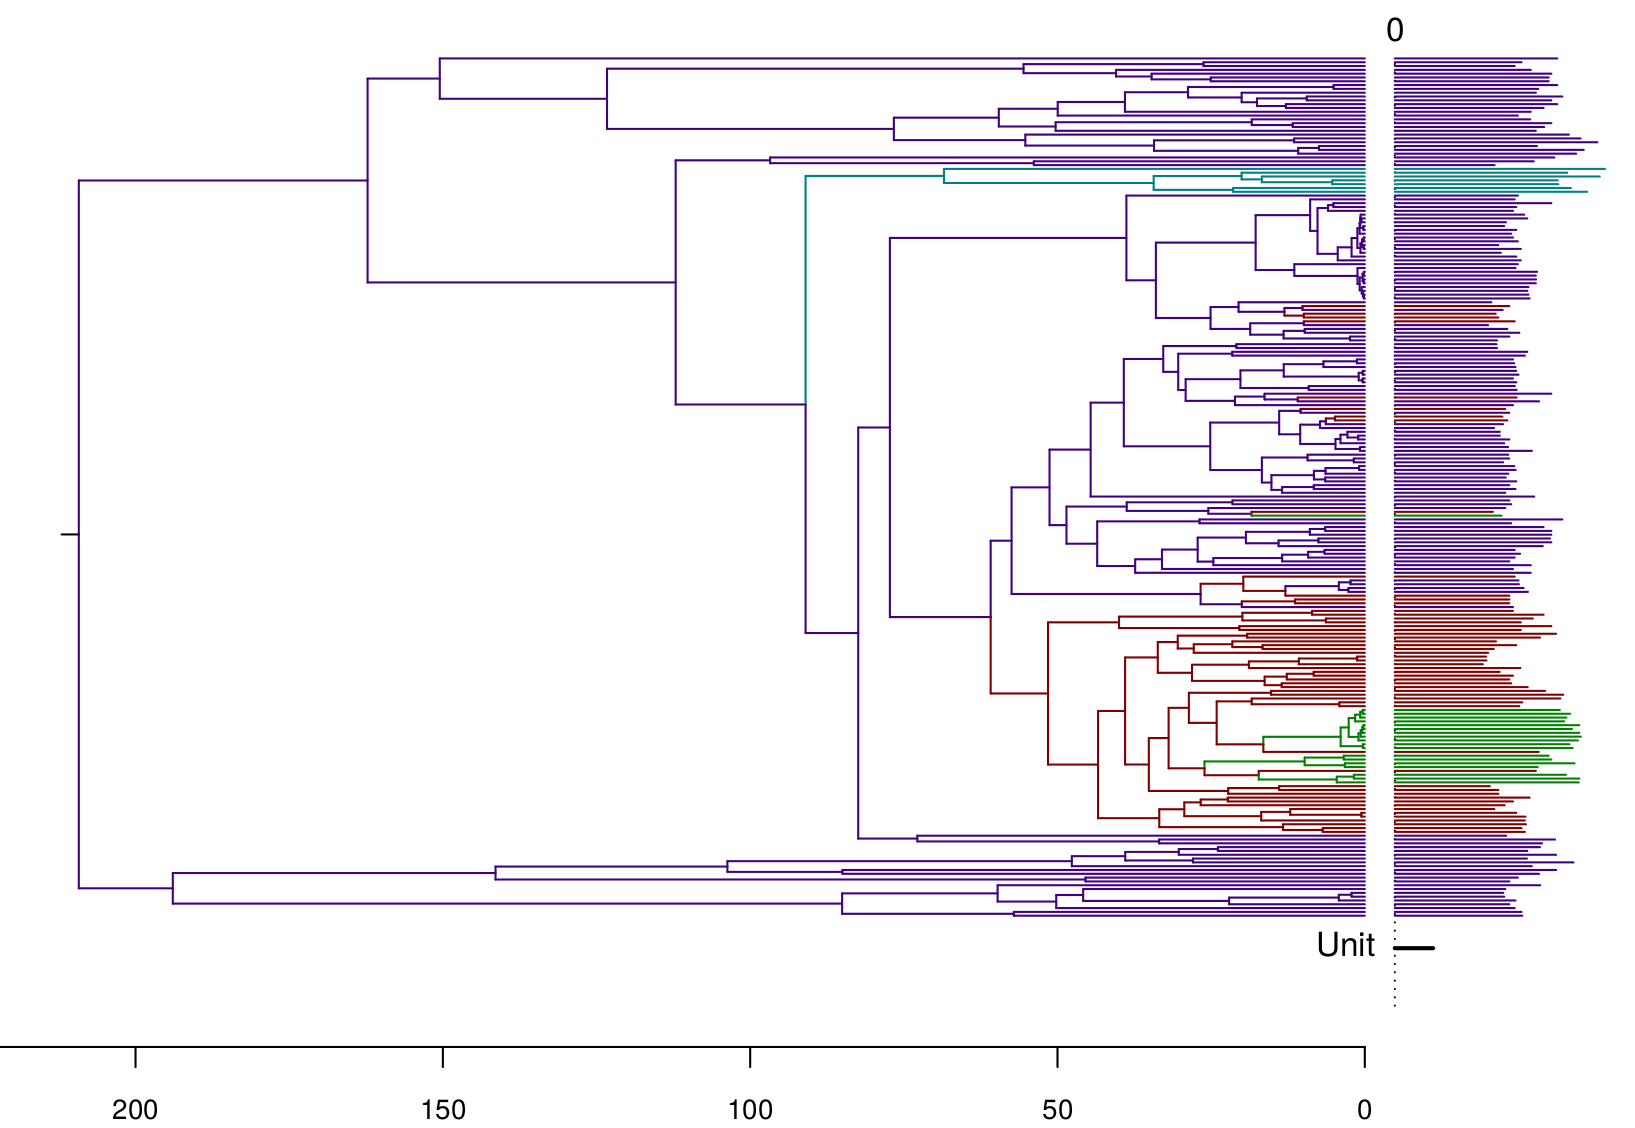
\includegraphics[width=.6\textwidth, clip=]{../FIGURES/plot_data_chel-intro-SR}
  $$
  \refer{JSA11}: Chelonia turtles, trait: carapace length 
  }

%====================================================================
\frame{\frametitle{A StatScale problem?}

  \paragraph{Problem.}
  \begin{itemize}
   \item Based on a \emphase{given} phylogenetic tree and on traits observed for \emphase{extant} species
   \item Infer adaptive shifts that may have occurred in the past
  \end{itemize}

  \bigskip \bigskip \pause
  \paragraph{A change-point problem.}
  \begin{itemize}
  \item Finding change-points in a stochastic process ... based only on end-points data
  \end{itemize}

  \bigskip \bigskip \pause
  \paragraph{Big data?}
  \begin{itemize}
  \item Medium number of species: several tens to few hundreds ... but data are collected every day
  \item Small number of traits: few tens ... but molecular data are coming
  \end{itemize} 
  
  ~ \\ 
  \ra Need for (reasonably) efficient algorithms
  }

%====================================================================
%====================================================================
\section{Evolution of one trait}
\frame{\frametitle{Outline} \tableofcontents[currentsection]}

%====================================================================
\subsection*{Model}
%====================================================================
\frame{\frametitle{Modeling the evolution of a trait}

  \paragraph{Generic model:} \refer{Fel85} 
   $$
  \includegraphics[width=.49\textwidth, clip=]{../FIGURES/plot_tree_tims_2-1}
  \includegraphics[width=.49\textwidth, clip=]{../FIGURES/plot_BM_sim_2-1}
   $$
   \vspace{-0.05\textheight}
   \begin{itemize}
   \item $X =$ random process going along the branches of the tree ; \\ ~
   \item at each internal nodes, independent copies bifurcate;s
   \end{itemize}
  }

%====================================================================
\frame{\frametitle{Introducing shifts}

   \vspace{-0.05\textheight}
   $$
   \includegraphics[width=.5\textwidth, clip=]{../FIGURES/plot_tree_tims_shift-1}
   \includegraphics[width=.5\textwidth, clip=]{../FIGURES/plot_BM_sim_shit-1}
   $$
   \vspace{-0.05\textheight}
   \begin{itemize}
   \item Same model as before; \\ ~
   \item Shifts occur at the start of some branches; \\ ~
   \item The distribution of the process is shifted accordingly.
   \end{itemize}
  }

%====================================================================
\frame{\frametitle{A first process: Brownian motion}

  \paragraph{Brownian motion (BM).} 
  $$
  \dd X(t) = \sigma \; \dd W(t)
  $$
  
  \bigskip \pause
  No memory \ra easy to understand and handle:
  \begin{align*}
    \Cov(X_A, X_B \;|\; X_{\text{Root}}) & = \sigma^2 t_{AB}, \\
    X_i \;|\; X_{\pa(i)} & \sim \Ncal(X_{\pa(i)} \emphase{+ \delta_i}, \sigma^2 \ell_i)
  \end{align*}

  \bigskip \pause
  But not stationary \ra unrealistic from an evolutionary point-of-view:
  $$   
  \Var(X(t) \;|\; X_{\text{Root}}) = \sigma^2 t
  $$

}

%====================================================================
\frame{\frametitle{Ornstein-Uhlenbeck process}

  \paragraph{Ornstein-Uhlenbeck (OU):} 
  $$
  \dd X(t) = \sigma \dd W(t) - \emphase{\alpha} \left(X(t) - \emphase{\beta}\right) \dd t
  $$
  \ra continuous-time version of the AR(1) process.
  
  \bigskip \bigskip \pause
  \begin{itemize}
   \item $\beta =$ 'optimum' value for the trait in a given niche \refer{Han97,BuK04} \\~
   \item $\alpha =$ recall strength toward $\beta$ \\~
   \item Stationary process with limit distribution
   $$
   \Ncal(\beta, \gamma^2), \qquad \gamma^2 = \sigma^2/2\alpha
   $$
  \end{itemize}
  
  }

%====================================================================
\frame{\frametitle{Ornstein-Uhlenbeck model with shifts}

  \paragraph{Adaptive shift:} Due to some environmental change, a shift occurs in the optimum
  \vspace{-0.05\textheight}
  $$
  \includegraphics[width=.5\textwidth, clip=]{../FIGURES/plot_tree_tims_shift-1}
  \includegraphics[width=.5\textwidth, clip=]{../FIGURES/plot_OU_sim_shit-1}
  $$
%   \vspace{-.1\textheight}
%   $$
% %   \vspace{-.1\textheight}
%   \includegraphics[width=.7\textwidth]{../FIGURES/plot_OU_sim_shit-1}
%   $$
  $$
  X_i | X_{\pa(i)} \sim \Ncal\left(X_{\pa(i)}e^{-\alpha \ell_i} + \beta_{i}(1 - e^{-\alpha \ell_i}), \frac{\sigma^2}{2\alpha} (1 - e^{-2\alpha \ell_i})\right)
  $$
}

%====================================================================
\frame{\frametitle{Reparametrization of the Ornstein-Uhlenbeck model}

  \paragraph{Property.} $X(t) =$ Ornstein-Uhlenbeck process, $W(t) = $ Brownian motion:
  $$
  X(t) = \sigma e^{-\alpha t} W(e^{2 \alpha t} - 1) / \sqrt{2 \alpha}
  $$
  
  
  \bigskip \bigskip \pause
  \paragraph{Consequence.} If $T$ is ultra-metric, we have 
  $$
  p_{\emphase{\OU}, \alpha}(X_A, X_B, \dots ; T) = p_{\emphase{\BM}}(X_A, X_B, \dots; \emphase{\widetilde{T}})
  $$
  where $\widetilde{T}$ is the \emphase{rescaled tree} with branch lengths
  $$
  \ell_i(\alpha) =  \frac{1}{2\alpha} e^{2-\alpha h} (e^{2\alpha t_i} - e^{2\alpha t_\pa(i)})
  $$
}

%====================================================================
\subsection*{Inference}
%====================================================================
\frame{\frametitle{Inference V1: Incomplete data model}

%   \hspace{-.055\textwidth}
  \paragraph{Complete data} $X = (Z, Y)$
  \begin{itemize}
  \item $(Z_i) = $ traits at the internal nodes (ancestors);
  \item $(Y_j) = $ traits at the leafs (extant species).
  \end{itemize}

  $$
  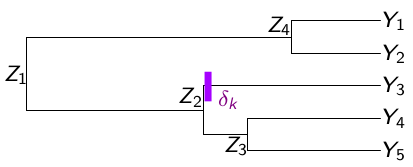
\includegraphics[width=.5\textwidth]{../FIGURES/IncompleteData-BMR15}
  $$
  
  \bigskip 
  \ra Standard inference algorithm = EM \refer{DLR77}
  $$
  \log p_\theta(X) = \sum_i \log p_\theta(X_i \;|\; X_{pa(i)}).
  $$
  }

%====================================================================
\frame{\frametitle{Inference V1: EM algorithm}

  \paragraph{E-step.} 2 ways to compute $p_{\theta^h}(X \; | \; Y)$
  \begin{enumerate}
   \item General properties of multivariate Gaussian (+ \refer{HoA13b}'s trick to invert $\Sigma_{YY}$).
   \item \emphase{Upward-downward} recursion taking advantage of the tree structure.
  \end{enumerate}
  
  \bigskip \bigskip \pause
  \paragraph{M-step.} The update of $\theta^h$ includes the \emphase{optimal allocation} of shifts to branches. \\~
  \begin{itemize}
  \item \pause BM: Two costs to compare for each branch
  \begin{eqnarray*}
  \text{without shift:} & & \Esp [\log \phi(X_j; X_{pa(j)}, \ell_j \sigma^2) | Y]\\
  \text{with shift:} & & \Esp [\log \phi(X_j; X_{pa(j)} \emphase{+ \delta_k}, \ell_j \sigma^2) | Y]
  \end{eqnarray*}
  \ra Trivial optimal allocation problem. \\~ 
  \item \pause OU: Use tree rescaling and proceed as for BM
  \end{itemize}
}

%====================================================================
\frame{\frametitle{Inference V2: Gaussian regression model}

  \begin{tabular}{cc}
    \begin{tabular}{p{.5\textwidth}}
	 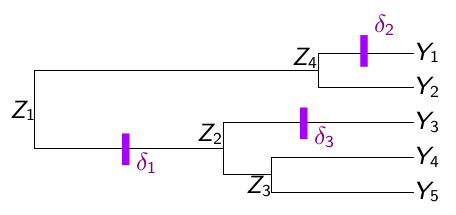
\includegraphics[width=.5\textwidth]{../FIGURES/RegressionView-BMR15}
    \end{tabular}
    & 
    \hspace{-.1\textwidth}
    \begin{tabular}{p{.5\textwidth}}
    {\scriptsize
    \[
    \Delta = \begin{bmatrix}
	 \mu\\ \delta_1\\ 0\\  0\\ \delta_2\\ 0\\ \delta_3\\ 0\\ 0\\
    \end{bmatrix}                           
    \qquad 
    T \Delta = \begin{bmatrix}
	 \mu + \delta_2\\ \mu\\ \mu + \delta_1 + \delta_3\\ \mu + \delta_1\\ \mu + \delta_1\\ 
    \end{bmatrix}
    \]
    }
    \end{tabular} 
    \\
    \begin{tabular}{p{.5\textwidth}}
         {\scriptsize
         \[
         \!\!\!T\!=\!
         \bordermatrix{
         \!&Z_1\!\!\!&Z_2\!\!\!&Z_3\!\!\!&Z_4\!\!\!&\!\!\!&Y_1\!\!\!&Y_2\!\!\!&Y_3\
         \!\!&Y_4\!\!\!&Y_5\cr
         Y_1\!&1&0&0&1&\!\!\!&1&0&0&0&0 \cr
         Y_2\!&1&0&0&1&\!\!\!&0&1&0&0&0 \cr
         Y_3\!&1&1&0&0&\!\!\!&0&0&1&0&0 \cr
         Y_4\!&1&1&1&0&\!\!\!&0&0&0&1&0 \cr
         Y_5\!&1&1&1&0&\!\!\!&0&0&0&0&1 \cr 
         }\]
         }
    \end{tabular}
    & 
    \hspace{-.1\textwidth}
    \begin{tabular}{p{.5\textwidth}}
    \begin{eqnarray*}
    Y & = & T\Delta + E \\
    E  & \sim & \Ncal(0, \Sigma) \\
    ~\\
    ( \Sigma & = & \Sigma_{YY})
    \end{eqnarray*}
    \end{tabular}
  \end{tabular}

  }

%====================================================================
\frame{\frametitle{Some more about the inference}

  \paragraph{Regression point of view:}
  \begin{itemize}
   \item Lasso initialization: 
   $$
   \arg\min_\delta \|Y - T\Delta\|^2_{\Sigma^{-1}} + \lambda |\Delta|;
   $$
   \item Identifiability issues: the null space of $T$ does not reduce to $0$;
   \item Useful representation for model selection.
  \end{itemize}

  \bigskip \bigskip \pause
  \paragraph{Ornstein-Uhlenbeck:} 
  \begin{itemize}
   \item Regression version
   $$
   Y = T W(\alpha) \Delta + E, \qquad E \sim \Ncal(0, \Sigma(\alpha))
   $$
   \ra Lasso intialization, identifiability and model selection still holds.
   \item Estimation of $\alpha$: 
   either within the EM loop, or externally, using a grid.
  \end{itemize}

}

%====================================================================
\frame{\frametitle{Identifiability}

  \begin{itemize}
   \item Shift allocation results in a coloring of the leafs. % (observable).
   \onslide+<2->{\item Some scenarios are parsimonious, some are not (homoplasy).}
   \onslide+<4->{\item Different scenarios may results in the same coloring.}
  \end{itemize}
  
  \begin{overprint}
   \onslide<3>
     \begin{tabular}{p{.25\textwidth}p{.05\textwidth}p{.25\textwidth}p{.05\textwidth}p{.25\textwidth}}
	 \begin{tabular}{c}
	 \includegraphics[width=0.15\textwidth]{../FIGURES/colours_1_nodes_gray} \\
	 2 colors \\ ~
	 \end{tabular}
	 & 
	 \begin{tabular}{c}
	 $:$
	 \end{tabular}
	 & 
	 \begin{tabular}{c}
	 \includegraphics[width=0.15\textwidth]{../FIGURES/colours_2_nodes_gray} \\
	 non \\
	 parsimonious
	 \end{tabular}
	 & 
	 \begin{tabular}{c}
	 $<$
	 \end{tabular}
	 & 
	 \begin{tabular}{c}
	 \includegraphics[width=0.15\textwidth]{../FIGURES/colours_3_nodes_gray} \\
	 parsimonious \\ ~
	\end{tabular}
  \end{tabular}
  \onslide<5>
     \begin{tabular}{p{.25\textwidth}p{.05\textwidth}p{.25\textwidth}p{.05\textwidth}p{.25\textwidth}}
	 \begin{tabular}{c}
	 \includegraphics[width=0.15\textwidth]{../FIGURES/colours_bis_1_nodes_gray} \\
	 3 colors
	 \end{tabular}
	 & 
	 \begin{tabular}{c}
	 $:$
	 \end{tabular}
	 & 
	 \begin{tabular}{c}
	 \includegraphics[width=0.15\textwidth]{../FIGURES/colours_bis_2_nodes_gray} \\
	 parsimonious
	 \end{tabular}
	 & 
	 \begin{tabular}{c}
	 $\sim$
	 \end{tabular}
	 & 
	 \begin{tabular}{c}
	 \includegraphics[width=0.15\textwidth]{../FIGURES/colours_bis_3_nodes_gray} \\
	 parsimonious
	\end{tabular}
  \end{tabular}
  \end{overprint}
}

%====================================================================
\frame{ \frametitle{Models with $K$ shifts}

  \paragraph{Assumption:} No homoplasy \ra 1 shift = 1 new color 
%   $$
%   K \text{ shifts} \quad \Leftrightarrow \quad K + 1 \text{ colors}
%   $$
 
  \bigskip \bigskip \pause
  \paragraph{Actual number of models:}
  \begin{itemize}
   \item $\Scal_K^P := \{\text{Parsimonious allocations of $K$ shifts}\}$ \\~
   \item Complexity of the $K$-shifts model class $= \# \Scal_K^{PI}$ where $\Scal_K^{PI} = \Scal_K^{P}/\sim$
  \end{itemize}


  \bigskip \bigskip \pause
  \paragraph{$\#{\Scal_K^{PI}}$ depends on the topology of the tree:}
  \begin{enumerate}
  \item $\#{\Scal_K^{PI}}$ can be computed recursively \refer{BMR16}. $\#{\Scal_K^{PI}} \leq \binom{m+n-1}{K}$. \\~
  \item For a binary tree: $\#{\Scal_K^{PI}} = \binom{2n-2-K}{K}$. \\~
  \item Parsimonious equivalent scenarios can be enumerated in $O(K^2Ln)$: generalization of \refer{Fit71,Fel04}\footnote{$L =$ max. number of offspring}
  \end{enumerate}

}

%====================================================================
\frame{ \frametitle{Example of equivalent scenarios}

  OU model: this 5 configurations only count for 1.
  $$
  \includegraphics[width=.8\textwidth]{../FIGURES/plot_parsimony-1}
  $$
}

%====================================================================
\frame{ \frametitle{Model selection: $K =$?}

  \paragraph{Specificity:} due to the discrete nature of the shift locations, standard criteria (AIC, BIC) do not apply.
  
  \bigskip \bigskip \pause
  \paragraph{Penalized criterion.} Under the BM model $Y = T \Delta + E$, $E \sim \Ncal(0, \Sigma)$, taking
  $$
  \widehat{\eta} = \arg\min_{\eta \in \Mcal} \|Y - \widehat{s}_\eta\|^2_{\Sigma^{-1}} + (1 + \text{Pen}(K_\eta))
  $$
  where
  $$
  \Mcal = \bigcup_{K \geq 0} \Scal^{PI}_K, 
  \qquad
  \text{Pen}(K) = f(n, K, \# \Scal^{PI}_K)
  $$
  ensures a non-asymptotic oracle inequality
%   ensures the oracle inequality
%   $$
%   \|Y - \widehat{s}_{\widehat{\eta}}\|^2_{\Sigma^{-1}}
%   \leq C_1 \left(\inf_{\eta \in \Mcal} \|s - \widehat{s}_\eta\|^2_{\Sigma^{-1}} + C_2(n, \eta) + C_3(n) \right)
%   $$

  \bigskip
  \begin{itemize}
   \item Proof adapted from \refer{BGH09}. 
   \item Generalizes to OU with known $\alpha$.
  \end{itemize}
}

%====================================================================
\subsection*{Illustration}
%====================================================================
\frame{ \frametitle{Back to Chelonia turtles}

  \only<1>{
    \begin{columns}
    \begin{column}{0.55\textwidth}
    \begin{minipage}[c][\textheight][c]{\linewidth}
    \vskip -1 cm
    \includegraphics[width=\linewidth]{../FIGURES/plot_chel_data1-1} \\
    {\footnotesize Colors: habitats.\\ Boxes: selected EM regimes.}
    \end{minipage}
    \end{column}
    \begin{column}{0.45\textwidth}
    \begin{minipage}[t][.6\textheight][c]{\linewidth}
    \end{minipage}
    \end{column}
    \end{columns}
    }
    \only<2>{
    \begin{columns}
    \begin{column}{0.55\textwidth}
    \begin{minipage}[c][\textheight][c]{\linewidth}
    \vskip -1 cm
    \includegraphics[width=\linewidth]{../FIGURES/plot_chel_data-1} \\
    {\footnotesize Colors: habitats.\\ Boxes: selected EM regimes.}
    \end{minipage}
    \end{column}
    \begin{column}{0.45\textwidth}
    \begin{minipage}[t][.6\textheight][c]{\linewidth}
    \vskip - 4 cm
    \includegraphics[width=0.5\textwidth]{../FIGURES/Chelonia_mydas.jpg} \\
    {\footnotesize Chelonia mydas}
    \end{minipage}
    \end{column}
    \end{columns}
    }
    \only<3>{
    \begin{columns}
    \begin{column}{0.55\textwidth}
    \begin{minipage}[c][\textheight][c]{\linewidth}
    \vskip -1 cm
    \includegraphics[width=\linewidth]{../FIGURES/plot_chel_data3-1}  \\
    {\footnotesize Colors: habitats.\\ Boxes: selected EM regimes.}
    \end{minipage}
    \end{column}
    \begin{column}{0.45\textwidth}
    \begin{minipage}[t][.6\textheight][c]{\linewidth}
    \includegraphics[width=0.5\textwidth]{../FIGURES/Geochelone_nigra_abingdoni.jpg} \\
    {\footnotesize Geochelone nigra abingdoni}
    \end{minipage}
    \end{column}
    \end{columns}
    }
    \only<4>{
    \begin{columns}
    \begin{column}{0.55\textwidth}
    \begin{minipage}[c][\textheight][c]{\linewidth}
    \vskip -1 cm
    \includegraphics[width=\linewidth]{../FIGURES/plot_chel_data5-1} \\
    {\footnotesize Colors: habitats.\\ Boxes: selected EM regimes.}
    \end{minipage}
    \end{column}
    \begin{column}{0.45\textwidth}
    \begin{minipage}[t][.6\textheight][c]{\linewidth}
    \vskip - 4 cm
    \includegraphics[width=0.5\textwidth]{../FIGURES/Dudhwalive_chitra.jpg} \\
    {\footnotesize Chitra indica}
    \end{minipage}
    \end{column}
    \end{columns}
    }
    \only<5>{
    \begin{columns}
    \begin{column}{0.55\textwidth}
    \begin{minipage}[c][\textheight][c]{\linewidth}
    \vskip -1 cm
    \hspace{.025\textwidth}
    \includegraphics[width=\linewidth]{../FIGURES/plot_chel_data4-1} \\
    {\footnotesize Colors: habitats.\\ Boxes: selected EM regimes.}
    \end{minipage}
    \end{column}
    \begin{column}{0.5\textwidth}
    \begin{minipage}[t][.6\textheight][c]{\linewidth}
    \vskip - 3 cm
    {\footnotesize
    \begin{table}[!ht]
    \begin{center}
    \begin{tabular}{l|c|c}
    \hline
    & Habitat & EM\\ \hline
    Nb shifts & 16 & 5\\ \hline
    Nb regimes & 4 & 6\\ \hline
    $\log P$ & -135.56 & -97.59\\ \hline
    $\ln 2 / \alpha$ (\%) & 7.83 & 5.43\\ \hline
    $\gamma^2$ & 0.35 & 0.22\\ \hline
%     CPU (mn) & 1.25 & 134.49\\ \hline
    \end{tabular}
    \end{center}
    \end{table}
    }
    \end{minipage}
    \end{column}
    \end{columns}
    }
}

%====================================================================
%====================================================================
\section{Joint evolution of correlated traits}
\frame{\frametitle{Outline} \tableofcontents[currentsection]}

%====================================================================
\frame{\frametitle{Multivariate correlated traits}

  \paragraph{Aim.}
  \begin{itemize}
  \item Several traits are often collected on each species:  $\Xbf_j = (X_{j1}, \dots X_{jp})$
  \item Adaptive shifts are likely to affect several of them
  \end{itemize}

  \bigskip \bigskip \pause
  \paragraph{Data at hand.}
  $$
  \Xbf = (X_{jk})_{j, k}: \quad n \times p \text{ data matrix}
  $$
  \begin{itemize}
  \item rows are correlated because of the phylogeny
  \item columns are correlated because morphologic traits are not independent
  \end{itemize}
}

%====================================================================
\subsection*{Model}
%====================================================================
\frame{\frametitle{Multivariate Ornstein-Uhlenbeck process}

  \paragraph{Phylogenetic PCA.} Under the BM model, 
  $$
  \Var[\text{vec}(\Ybf)] = \Cbf \otimes \Rbf
  $$
  where $\Cbf = [t_{ij}]$, $\Rbf$ the between trait covariance matrix.
  
  \bigskip
  \begin{itemize}
   \item Phylogenetic PCA \refer{Rev09} allows to decorrelate the traits accounting for the phylogenetic dependence 
   \item ... in absence of shifts (between-within cluster variances are confounded)
  \end{itemize}
  
  \bigskip \pause
  \paragraph{Multivariate OU process.}
  $$
  \dd \Xbf(t) = \Abf(\betabf - \Xbf(t)) \dd t + \Rbf \; \dd \Wbf(t)
  $$
  where  
  \begin{itemize}
  \item $\Wbf(t) =$ standard multivariate BM,
  \item $\betabf =$ vector of optimums,
  \item $\Abf =$ matrix of recall strengths.
  \end{itemize}
}


%====================================================================
\subsection*{Inference}
%====================================================================
%====================================================================
\frame{\frametitle{Inference}

  \paragraph{Simplifying assumptions} to ensure tractable inference.
  \begin{itemize}
   \item $\ell1$ou \refer{KKR16}: arbitrary $\Abf$, diagonal $\Rbf$ \ra independent traits;
   \item scOU \refer{BAR18}: arbitrary $\Rbf$, $\Abf = \alpha \Ibb$ \ra same recall strength for all traits.
  \end{itemize}

  \bigskip \bigskip \pause
  \paragraph{'Scalar' OU (scOU) process with shifts.}
  $$
  \Xbf_j \;|\; \Xbf_{\pa(j)} \sim \Ncal\left(e^{\alpha \ell_j} \Xbf_{\pa(j)} + (1 - e^{\alpha \ell_j}) \betabf_j; \frac1{2\alpha} (1 - e^{\alpha \ell_j}) \Rbf \right)
  $$

  \bigskip \bigskip \pause
  \paragraph{Inference via EM.} Similar to 1D:
  \begin{itemize}
   \item Tree rescaling (for given $\alpha$) \ra straightforward shift location,
   \item Upward-downward recursion (to avoid $np \times np$ matrix manipulation),
   \item Preliminary PCA can be useful for numerical reasons.
  \end{itemize}


}

%====================================================================
\subsection*{Illustration}
%====================================================================
%====================================================================
\frame{\frametitle{Of monkeys and lizards}

  \paragraph{Monkey brain shape.} %\refer{ADM16}
  \begin{itemize}
   \item $n =49$ new world monkey species
   \item Traits = PC1 and PC2 from 399 landmarks describing brain shapes
   \item First analyzed by \refer{ADM16}
  \end{itemize}
  
  \bigskip \bigskip 
  \paragraph{Lizard} %\refer{MIR13}
  \begin{itemize}
   \item $n =100$ island lizard species
   \item Traits = 11 morphological measurements
   \item First analyzed by \refer{MIR13}
  \end{itemize}

  }	

%====================================================================
\frame{\frametitle{Monkeys}

    \begin{tabular}{cc}
    \begin{tabular}{p{.4\textwidth}}
	 Top: scOU, bottom: \refer{ADM16}
    
	 \bigskip \bigskip 
      Results mostly consistent except \\
      \begin{itemize}
      \item (\textcolor{green}{$\nabla$}, $\square$) / $\square$: no significant
      difference \\~
      \item (\textcolor{red}{$*$}, \textcolor{red}{$\times$}) / \textcolor{red}
      {$\times$}: no homoplasy \\~
      \item color of the top branches: no use of the fossil record
      \end{itemize}
    \end{tabular}
    & 
    \hspace{-.02\textwidth}
    \begin{tabular}{p{.5\textwidth}}
	 \includegraphics[width=.6\textwidth, height=.6\textheight, clip=, angle=270]{../FIGURES/BAR18-SystBiol-Fig10}
    \end{tabular}
  \end{tabular}

%   $$
%   \includegraphics[width=.8textwidth, clip=]{../FIGURES/BAR18-SystBiol-Fig10}
%   $$
%   Results mostly consistent except
%   \begin{itemize}
%    \item (\textcolor{green}{$\nabla$}, $\square$) / $\square$: no significant difference
%    \item (\textcolor{red}{$*$}, \textcolor{red}{$\times$}) / \textcolor{red}{$\times$}: no homoplasy
%    \item color of the top branches: no use of the fossil recors
%   \end{itemize}

}

%====================================================================
\frame{\frametitle{\url{PhylogeneticEM} package}

  \paragraph{Equivalent shift locations.}
  \begin{itemize}
  \item {\tt eq\_shifts <- equivalent\_shifts(phylogeny, params\_5)} 
  \item {\tt plot(eq\_shifts, ...)}
  \end{itemize}
  
  $$
  \includegraphics[width=.9\textwidth]{../FIGURES/BAM17-SupMat-Fig3}
  $$
}

%====================================================================
\frame{\frametitle{Lizards}

  $$
  \includegraphics[width=.5\textwidth, clip=, angle=270]{../FIGURES/BAR18-SystBiol-Fig12}
  $$
  \begin{itemize}
  \item Due to high correlations between traits, pseudo-orthogonalization is needed
  \end{itemize}

}

%====================================================================
\section{Conclusion and future work}
\frame{\frametitle{Outline} \tableofcontents[currentsection]}
%====================================================================
\frame{\frametitle{Conclusion \& Future works}

  \paragraph{Conclusions.}
  \begin{itemize}
   \item Comprehensive statistical framework: 
   (multivariate) OU model with shifts \\
   + EM algorithm + identifiability + model selection;
   \item R package \url{Phylogenetic-EM};
   \item \refer{BMR16,BAR18}
  \end{itemize}

  \bigskip \bigskip \pause
  \paragraph{Future work.}
  \begin{itemize}
%    \item 'Spasify' the multivariate version so that not all traits are affected by each shift;
   \item Can we deal with non ultrametric tree?
   \item Consider fossil records to distinguish between equivalent scenarios.
   \item Deal with the uncertainty of the tree.
   \item Deal with non tree-shaped evolution ('network' because of hybridization and horizontal transfers).
  \end{itemize}

}

%====================================================================
\frame[allowframebreaks]{ \frametitle{References}

% \nocite{BMR16,BAR17}
{\tiny
  \bibliography{/home/robin/Biblio/BibGene}
%   \bibliographystyle{/home/robin/LATEX/Biblio/astats}
  \bibliographystyle{alpha}
  }
}

%====================================================================
\appendix 
\backupbegin
\section{Appendix}

%====================================================================
\frame{\frametitle{Notations}
  
  $$
  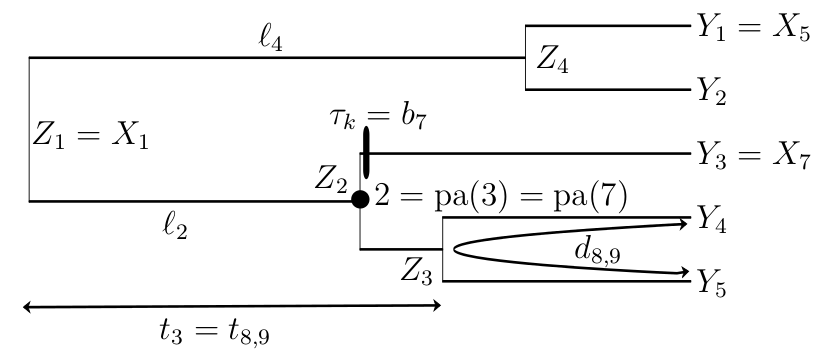
\includegraphics[width=.8\textwidth]{../FIGURES/Notations-BMR15}
  $$
  }
  
%====================================================================
\frame{\frametitle{Computation time}
  
  $$
  \includegraphics[width=.6\textwidth]{../FIGURES/BAR18-Fig8}
  $$
  \begin{itemize}
   \item 4 traits.
   \item High-performance computing facility with CPU speed 2.5 GHz.
  \end{itemize}
  }
  
%====================================================================
\backupend

%====================================================================
%====================================================================
\end{document}
%====================================================================
%====================================================================

  \begin{tabular}{cc}
    \begin{tabular}{p{.5\textwidth}}
    \end{tabular}
    & 
    \hspace{-.02\textwidth}
    \begin{tabular}{p{.5\textwidth}}
    \end{tabular}
  \end{tabular}

